\documentclass[a4paper,12pt,oneside,openany,table,xcdraw]{article}

\usepackage{setspace}
\usepackage{multirow}
\usepackage{hyperref}
\usepackage{caption}
\usepackage{indentfirst}

\usepackage[brazilian]{babel}
\usepackage[utf8x]{inputenc}
\usepackage{amsmath, graphicx, enumerate}
\usepackage{float, verbatim}
\usepackage[colorinlistoftodos]{todonotes}
\usepackage{makeidx} % Para o sumário
\usepackage{geometry}

\usepackage{mathtools,listings}

\geometry{a4paper, hmargin={3cm, 3cm}, vmargin={3cm, 2cm} }
\setlength{\parindent}{1.0cm}

\begin{document}
\newcommand{\thedepartment}{Faculdade de Engenharia Elétrica}
\newcommand{\thecourse}{FEELT}
\newcommand{\thetitle}{LISTA DE EXERCÍCIOS EXTRAS}
\newcommand{\thetype}{Relatório da Disciplina de Sinais e Sistemas 2}
\newcommand{\theproftitle}{Doutor em Engenharia Elétrica com ênfase em Telecomunicações}
\newcommand{\thestudent}{Lesly Viviane Montúfar Berrios\\
\centering11811ETE001}
\newcommand{\theadvisor}{Prof. Alan Petrônio Pinheiro}
\newcommand{\thecity}{Uberlândia}

\thispagestyle{empty}\newcommand*{\themonth}{\ifthenelse{\the\month < 2}{Janeiro }
                  {\ifthenelse{\the\month < 3}{Fevereiro }
                  {\ifthenelse{\the\month < 4}{Março }
                  {\ifthenelse{\the\month < 5}{Abril }
                  {\ifthenelse{\the\month < 6}{Maio }
                  {\ifthenelse{\the\month < 7}{Junho }
                  {\ifthenelse{\the\month < 8}{Julho }
                  {\ifthenelse{\the\month < 9}{Agosto }
                  {\ifthenelse{\the\month < 10}{Setembro }
                  {\ifthenelse{\the\month < 11}{Outubro }
                  {\ifthenelse{\the\month < 12}{Novembro }{Dezembro }}}}}}}}}}}}
                  
\begin{titlepage}
\begin{center}

	\vspace{-0.5cm}

  \begin{figure}[hbt!]
		\begin{center}
		   
\includegraphics[width=2.8cm]{ufu-logo.png}
		\end{center}
	\end{figure}
 	%\vspace{-4cm}

%\begin{doublespacing}

  \Large{\textbf{Universidade Federal de Uberlândia}}\\
  \large{\thedepartment}\\
  \large{\thecourse}\\


\vspace{5.8cm}
  \par
  \large\textbf{\thetitle}
\vspace{5.8cm} 

%\end{doublespacing}
  \par
  \thetype\\
  por\\
  %\hspace{2cm}\large{}\\

\vspace{0.8cm}
\par
  \normalsize{\thestudent}\\ [2cm]
  \theadvisor

\par\vfill
  \thecity, \themonth / \the\year

\end{center}

\end{titlepage}

%% Comeca o documento !

\onehalfspacing
\tableofcontents % sumário
\newpage

\section{Exercício 1}
A resolução do item \textbf{a} visualiza-se na Figura \ref{scan:1a}.

\begin{figure}[H]
\centering
\captionsetup{font=scriptsize}
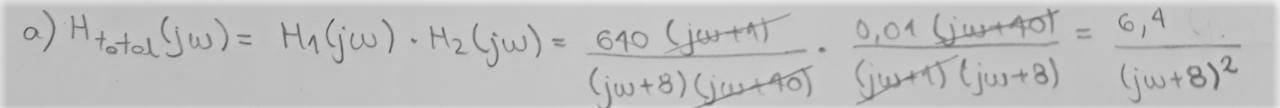
\includegraphics[width=14.5cm]{1a}
\caption{Resolução do item \textbf{a}.}
\label{scan:1a}
\end{figure}



\subsection{c)}
Sabemos que:
\begin{center}
    $x_p(t) = x(t) * p(t)$\\
    \vspace{0.25cm}
\end{center}

Logo, temos:
\begin{center}
    $$p(t) = \sum_{k=- \infty}^{\infty} \delta(t - nT)$$\\
    \vspace{0.25cm}
    $$p(t) = \sum_{k=- \infty}^{\infty} x(nT) \times \delta(t - nT)$$\\
    \vspace{0.25cm}
\end{center}

Portanto, podemos concluir:
\begin{center}
    $$p(t) = \sum_{k=- \infty}^{\infty} x(0,002T) \times \delta(t - 0,002T)$$\\
\end{center}


\subsection{d)}
Obtemos $X_p(j\omega)$ a partir da propriedade da multiplicação, onde:
\begin{center}
    $$X_p(j\omega) = \int_{-\infty}^{\infty} X(j\theta)P(j(\omega - \theta)) d\theta$$\\
\end{center}
E, sabendo que:
\begin{center}
    \vspace{0.25cm}
    $$P(j\omega) = \frac{2\pi}{T} \sum_{k=- \infty}^{\infty} \delta(\omega - k\omega_s)$$\\
    \vspace{0.25cm}
\end{center}
Assim, obtemos um resultado do tipo:
\begin{center}
    \vspace{0.25cm}
    $$X_p(j\omega) = \frac{1}{T} \sum_{k=- \infty}^{\infty} X(j(\omega - k\omega_s))$$\\
    \vspace{0.25cm}  
\end{center}

Sendo $\omega_s = \frac{2\pi}{T}$, podemos concluir que $X_p(j\omega)$ é:

\begin{center}
    \vspace{0.25cm}
    $$X_p(j\omega) = 500 \sum_{k=- \infty}^{\infty} X(j(\omega - 3141,59k))$$\\
    \vspace{0.25cm} 
\end{center}

Uma vez que é notável que o resultado foi obtido através do processo de convolução de $X(j\omega)$ com uma série de impulsos, podemos concluir que $X_p(j\omega)$ trata-se de uma função periódica que consiste na sobreposição de réplicas deslocadas de $X(j\omega)$

\subsection{e)}

 Um retentor de ordem zero (ZOH) amostra $x(t)$ em determinado instante e mantém esse valor até o próximo instante no qual a amostra é tomada. Portanto, podemos construí-lo a partir de filtragem passa-baixa.\\
 A partir da saída $x_0(i)$ do ZOH, obtemos a característica de filtro exigida. A resposta $H_0(j\omega)$ é:
 
 \begin{center}
     $H_0(j\omega) = e^{-j\omega T/2}\bigg[\frac{2sen(\omega T/2)}{\omega}\bigg]$
 \end{center}

E isso requer:


 \begin{center}
     $$H_r(j\omega) = \frac{e^{-j\omega T/2}H(j\omega)}{\frac{2sen(\omega T/2)}{\omega}}$$
 \end{center}
Por fim, temos

\begin{center}
    $H_0(j\omega) = e^{-j0,001\omega}\bigg[\frac{2sen(0,001\omega)}{\omega}\bigg]$
    
\end{center}

\subsection{f)}

Como anuncia o Teorema da Amostragem, um sinal $x(t)$ com banda limitada para um valor de $|\omega| > \omega_M$ é determinado por suas amostras $x(nT); n = 0, \pm1, \pm2, ...$

Para realizar um processo de recuperação do sinal amostrado, a frequência deve ser maior que $2\omega_M$. Essa frequência de amostragem é conhecida como taxa de Nyquist.

Portanto, temos que $\omega_s > 2\omega_M$

Para o sinal amostrado, o valor de $\omega_M$ pode ser calculado:

\begin{center}
    $$\omega_M = \frac{2\pi}{T} = 125,66 rad/s$$
\end{center}

Logo, a frequência de Nyquist deve ser

\begin{center}
    $$\omega_s > 2\omega_M = 251,32 rad/s$$
\end{center}

\subsection{g)}
Quando a frequência adotada para amostragem não satisfaz a frequência de Nyquist, ocorro o que é chamado de Aliasing. Réplicas deslocadas do sinal acabam por sobrepor umas as outras, tornando menos eficaz o processo de recuperação do sinal. Por isso, utiliza-se um filtro anti-aliasing que limita a banda para satisfazer a condição para que então efetue-se após a amostragem adequada, prevenindo a chance da formação do aliasing.

\subsection{h)}

\begin{figure}[H]
    \centering
    
\includegraphics[width=0.85\textwidth]{a}
    \caption{Diagrama de blocos}.
    \label{fig:my_label}
\end{figure}

\subsection{i)}


O valor $a_0$ da série de Fourier pode ser interpretado como um valor médio do sinal para um período. Analisando os valores de máximos e mínimos locais, visíveis na figura do sinal fornecido, é possível estimar que o valor de $a_0$ é próximo de 20.

Entretanto, para o cálculo de $a_k$, é necessário que a função do sinal seja conhecida. $a_0$ é calculado da seguinte forma:

\begin{center}
    $$a_k = \frac{1}{T}\int_{T}^{} x(t)e^{-jk(2\pi/T)} dt$$\\
\end{center}


\section{Exercício 3}

\subsection{a)}

A função subplot cria eixos para o gráfico a ser criado. Na froma subplot(m,n,p), temos uma rede m por n, sendo que m e n definem o tamanho dos eixos, e p determina a posição para a criação dos eixos.  

\subsection{b)}

A função ezplot é utlizada pra criar gráficos bidimensionais. A função gera um gráfico de uma expressão simbólica, ou função de f. Se os intervalos não forem predefinidos quando a função é chamada, o intervalo padrão é $[–2\pi 2\pi]$.

\subsection{c)}

O comando axis tem como função definir eixos a seres exibidos. por padrão, o comando não é requisito para a criação de um gráfico, mas é essencial para personalizar os eixos deste. 

\subsection{d)}

É observável que o período adotado é $T = 0,05$.\\

O comando $t = 0:T:1$ define t de maneira que t varie de 0 até 1, sendo que cada unidade da escala tem o valor de $T$, ou seja, 0,05.

\subsection{e)}

O comando Stem cria uma sequência discreta de impulsos. Se definida, uma função qualquer pode ser argumento da função Stem, de modo que o gráfico resultante seja uma representação discreta da função original.

\subsection{f)}

O comando stairs cria, a partir de uma função qualquer definida como argumento da função, uma representação em degraus da função inicial.

\subsection{g)}

Para a primeira amostragem, foi utilizado um período de amostragem de $T = 0,05$

\begin{figure}[H]
    \centering
    
\includegraphics[width=0.85\textwidth]{a}
    \caption{$T = 0,05$}.
    \label{fig:my_label}
\end{figure}

Para a segunda amostragem, foi utilizado um período de amostragem de $T = 0,20$

\begin{figure}[H]
    \centering
    
\includegraphics[width=0.85\textwidth]{a}
    \caption{$T = 0,20$}.
    \label{fig:my_label}
\end{figure}

Podemos observar que, como a frequência de $f_2(t)$ é maior do que a frequência de $f_1(t)$, o período de amostragem para uma melhor recuperação deve ser menor do que o período exigido por $f_1(t)$.

\section{Exercício 4}
\subsection{a)}
Para as funções $f_1(t)=e^{-0.5t}u(t)$, $f_2(t)=sin(2\pi t)$ e $f_3(t)=sin(2\pi2t)$ as transformadas calculadas pelo MATLAB foram:
\begin{itemize}
    \item $F_1(j\omega)=\frac{1}{1/2 + j\omega}$
    \item $F_2(j\omega)=-\frac{j}{\pi}[\delta(\omega-2\pi)+\delta(\omega-2\pi)]$
    \item $F_3(j\omega)=-\frac{j}{\pi}[\delta(\omega-4\pi)+\delta(\omega-4\pi)]$
\end{itemize}

\subsection{b)}
Para as funcões $F_4(j\omega)=\frac{2sen(0.002\omega)}{\omega}$, $F_5(j\omega)=2 \pi \delta(\omega)$, $F_6(j\omega)=2 \pi \delta(\omega-2)$ e $F_7(j\omega)=\pi[\delta(\omega-2 \pi)+\delta(\omega+2 \pi)]$ as transformadas inversas de Fourier calculadas pelo MATLAB foram:
\begin{itemize}
    \item $f_4(t)= \delta(1,x-0.002) + \delta(1,x+0.002)$
    \item $f_5(t)=1$
    \item $f_6(t)=e^{2j\omega}$
    \item $f_7(t)=cos(2 \pi t)$
\end{itemize}

\subsection{c)}

Para o a função $H_0(j \omega)$ calculada no item 2.e) temos os gráficos de magnitude e fase representados na figura a seguir.
\begin{figure}[H]
    \centering
    
\includegraphics[width = 0.85 \textwidth]{a}
    \caption{Magnitude e fase de $H(j \omega)$}
    \label{fig:my_label}
\end{figure}

\section{Exercício 5}
\subsection{a)} 
Para a resposta em frequência $H_1(j\omega)=\frac{1}{(j\omega)^2+4(j\omega)+4}$, temos o sistema:\\ $\frac{d^2y(t)}{dt^2}+4\frac{dy(t)}{dt}+4y(t)=x(t)$
\newline \newline
A frequência natural não amortecida $\omega_n = \sqrt{4} = 2$.
\newline
$2\omega_n\zeta=4 \Longrightarrow \zeta = 1$. Como $\zeta=1$, o sistema é \textbf{criticamente amortecido}.\newline \newline

\begin{figure}[H]
    \centering
    
\includegraphics[width=0.85\textwidth]{a}
    \caption{Gráficos de Bode de magnitude e fase de $H_1(j\omega)$}.
    \label{fig:my_label}
\end{figure}

\subsection{b)}
Para a resposta em frequência $H_2(j\omega)=\frac{7}{5(j\omega)^2+4(j\omega)+5}$, temos o sistema:\\
$5\frac{d^2y(t)}{dt^2}+4\frac{dy(t)}{dt}+5y(t)=7x(t)$.\newline
\newline
A frequência natural não amortecida é $\omega_n = \sqrt{5} \approx 2.23607$.
\newline
$2\omega_n\zeta=4 \Longrightarrow \zeta \approx 0.94427$.Como $\zeta<1$, o sistema é \textbf{subamortecido}.

\begin{figure}[H]
    \centering
    
\includegraphics[width=0.85\textwidth]{a}
    \caption{Gráficos de Bode de magnitude e fase de $H_2(j\omega)$}.
    \label{fig:my_label}
\end{figure}


\end{document}